\documentclass[a4paper]{report}
% \documentclass[a4paper,twoside,openright]{report}
% \documentclass[a4paper]{book}

%% Spanska!
\usepackage[utf8]{inputenc}
\usepackage[T1]{fontenc}    % 8-bit encoding. Acentuados como único caracter.
\usepackage[spanish, es-tabla]{babel}
% \def\spanishoptions{argentina}

%% graphics
\usepackage{graphicx}
\graphicspath{ {./graphs/} }
\usepackage{wrapfig}

%% biblatex
\usepackage[style=numeric, backend=biber, sorting= none, url= true, maxnames=20]{biblatex}
\DefineBibliographyStrings{spanish}{}
\usepackage{csquotes}
\usepackage{textgreek} % https://tex.stackexchange.com/questions/107352/non-ascii-characters-in-biblatex 
\addbibresource{sismos.bib}

%% physics
\usepackage[separate-uncertainty=true, locale=FR]{siunitx}

%% vínculos en documento pdf
\usepackage{hyperref}
\usepackage[all]{hypcap}
\hypersetup{
    colorlinks=false    % false:boxedlinks ; true:coloredlinks
}



\begin{document}

\title{
	{Factores de percepción de terremotos en Argentina}\\[1 cm]
	{Trabajo final de la asignatura ``Taller de tesis''}
	{
\includegraphics[width=\textwidth]{logos}}
}
\author{Víctor A. Bettachini}
\date{\today}
\maketitle

\begin{abstract}
	Niente.
\end{abstract}

\tableofcontents

% \mainmatter

\chapter{Introducción}

\section{Contexto y motivación científica}

Un rápido desprendimiento entre dos fascetas enfrentadas de sendas placas tecnónicas que trabanban mutuamente su desplazamiento relativo produce una rápida liberación de energía que se denomina terremoto.
Esto sucede a cierta profundidad en la corteza terrestre en el punto denominado hipocentro a partir del cual parte de esta energía se encauza como ondas elásticas.
El estudio de estas ondas es el área llamada sismología y de ahí el termino sismo para un evento particular detectado, pero que debiera aclararse si se produjo por un terremoto u otra fuente de ondas \cite[sección 4.1.1]{fowler_solid_2004}.
Sea que las ondas sean de compresión longitudinal de la corteza, las tipo P, o las del tipo S transversales y más lentas, ambas arriban con mayor intensidad al punto de la superficial terrestre que se encuentra directamente sobre el hipocentro, que se denomina epicentro \cite[sección 4.1.2]{fowler_solid_2004} como ilustra la figura \ref{fig:epicentro_hipocentro}.
\begin{wrapfigure}[13]{r}{0.4\textwidth}
  \centering
	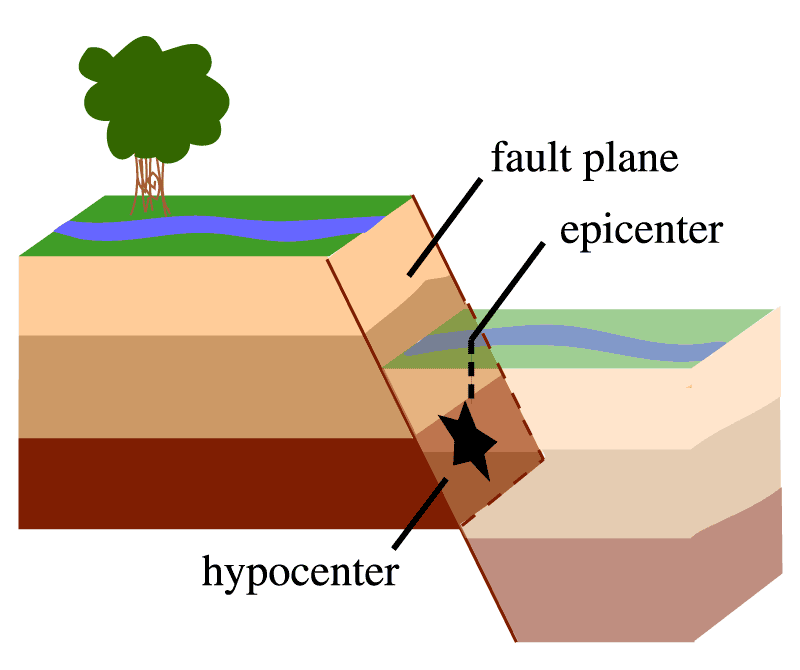
\includegraphics[width=0.3\textwidth]{eq-ed-fault-labeled.png}
	\caption{Epicentro e hipocentro de un sismo.}
	\label{fig:epicentro_hipocentro}
\end{wrapfigure}
Cuanto más proxima es una locación en la superficie a un epicentro la amplitud de las ondas sísmicas es mayor.
Tanto esta amplitud como el período de oscilación son mucho mayores que el de otros desplazamientos de la corteza respecto a otros desplazamientos como los de las mareas solares y lunares de la corteza \cite[sección 4.1.4]{fowler_solid_2004}.
Como resultado estructuras artificiales pueden agitarse poniendo en riesgo su estabilidad estructural y haciendo caer elementos que no estaban fijados a esta o perdieron tal adhesión a causa de la agitación misma.
Como consecuencia los sismos más fuertes pueden generar graves daños, poniendo en riesgo la integridad física y la seguridad de las personas al generar daños en las viviendas y edificios, derrumbes de puentes, rompimiento de vidrios, entre otros \cite{noauthor_que_2018}.

Pero de hecho la mayor parte de los sismos son de muy pequeña magnitud y no generan daños materiales.
Sin embargo el que sean o no detectados por la población es un factor relevante en su percepción de confianza vis-à-vís de los organismos de monitoreo y prevención de riesgos.
Sí o cuando informar a la población de la ocurrencia de un sismo es una decisión de política pública que debiera apuntar a no alertar  innecesariamente sobre sismos menores imperceptibles \cite{saunders_j_k_twist_nodate}.
El caso inverso es también problemático con casos en que ante una carencia de una comunicación oficial de la poca importancia de un evento sismico llevó a la autoevacuación por parte de la población que lo percibió \cite{vaiciulyte_population_2022}. 


\section{Objetivos del trabajo / Pregunta}
Contar con una estimación rápida a partir de los datos sismicos registrados por instrumental de si un dado evento será percibido por la población o no permitiría a las autoridades tomar decisiones informadas sobre la comunicación a la población.
Este trabajo busca determinar si con métodos de ciencias de datos puede predecirse con un grado de certeza elevado si un sismo será percibido por la población o no a partir de las variables de los sismos que se registran en los datos del Instituto Nacional de Prevención Sísmica (INPRES) que es el organismo público de Argentina que realiza estudios e investigaciones básicas y aplicadas de sismología \cite{noauthor_instituto_2022}.



\section{Estructura del documento}

Se estructuró en los siguientes capitulos con temáticas difenciadas
\begin{description}
	\item[Introducción]: se presentará el contexto y la motivación científica, los objetivos del trabajo y la estructura del documento.
	\item[Marco teórico]: se revisarán los trabajos previos y relevantes, se presentarán los conceptos y técnicas de ciencia de datos utilizados en el trabajo.
	\item[Metodología]: se describirán los datos utilizados, el preprocesamiento y limpieza de los mismos, el análisis exploratorio de los datos, las técnicas de análisis y modelado utilizadas, la selección de características, las métricas de evaluación de los modelos y los métodos estadísticos utilizados.
	\item[Resultados y discusión]: se presentarán y analizarán los resultados obtenidos, se discutirán los resultados y su relevancia, se identificarán las limitaciones y posibles mejoras.
	\item[Conclusión]: se resumirán los hallazgos principales, se presentarán las conclusiones generales y su relación con los objetivos del trabajo, se discutirán las aplicaciones y relevancia de los resultados.
\end{description}



\chapter{Marco teórico}

\section{Relevamiento de trabajos previos y relevantes}





\section{Conceptos y técnicas de ciencia de datos utilizados en el trabajo}
Siendo el objetivo de cualquier modelo utilizado una clasificación entre dos clases, la percepción de un sismo o no, se busca determinar que tan fuerte es el vínculo de cada una de las variables de los sismos de las que se dispone datos y la percepción de los mismos por parte de la población.
Para esto dos técnicas se planea utilizar dos distintas técnicas de la ciencia de datos: la regresión logística y la clasificación de árboles de decisión. 

Un modelo de regresión logística permite una clasificación binaria de los datos en función de una variable dependiente y un conjunto de variables independientes al tiempo de dar un peso a cada una de estas últimas lo que permitirá transmitir cuales son más relevantes en la clasificación.
Determinar la atribución de la percepción de un sismo a las variables de los mismos se considera de interés para los objetivo de este trabajo. 
Ajustando el grado de regularización tipo Lasso (L1) se buscará reducir el número de variables independientes en el modelo verificando en que grado su omisión afecta a la predicción.

Por otra parte se buscará utilizar una herramienta más reciente, las máquinas de potenciacion de gradiente, más conocidos por su nombre en inglés Gradient Boosting Machines (GBM).
Las distintas implementaciones de estos algoritmos, como XGBoost, LightGBM o CatBoost son capaces de producir un único modelo con fuerte poder predictivo a partir de la síntesis de resultados de modelos de predicción débiles, típicamente árboles de decisión. 
% Se planea utilizar la implementación de XGBoost en lenguaje R para este trabajo.

Puesto que los GBM carecen de un mecanísmo para evidenciar la importancia de las variables en la clasificación como la que evidencian los pesos de la regresión logística, se planea utilizar los valores de explicaciones aditivas de Shapley (SHapley Additive exPlanations, SHAP) para tal fin.
Para el lenguaje R está disponible la biblioteca \emph{shapr} para tal fin \cite{camilla_lingjaerde_shapr_nodate}.

El disponer de una herramienta de explicación de los modelos de predección aplicable al resultado de los dos a ensayar, el de regresión lógistica y el XGBoost, permitirá comparar la relevancia de las variables que asignará cada uno para la percepción de los sismos por parte de la población.



\chapter{Metodología}

\section{Presentación y descripción de los datos utilizados}

En el marco de los ``Proyectos de Asistencia Estadística del Instituto de Cálculo (IC)'' de la Facultad de Ciencias Exactas y Naturales (FCEyN) de la Universidad de Buenos Aires (UBA) se publicaron conjuntos de datos en un repositorio curado con el objeto de ser aplicados a la enseñanza de la estadística y la ciencia de datos por Daniela Parada, investigadora del IC \cite{noauthor_ic-datasets-docencia_nodate}.
De estos conjuntos el utilizado en este trabajo es el que se publica en el apartado ``Visualización'' que corresponden a datos de sismos de Argentina de los últimos 10 años \cite{daniela_parada_ic-datasets-docencia_nodate}. 
En este repositorio alojado por la firma GitHub, se provee un front-end html que da un contexto, hace una exploración inicial, un analísis para una provincia en particular, muestra una estimación de probabilidad y provee otra información sobre lo datos.

Los datos corresponden a detecciones por parte de estaciones de monitoreo sísmico en la República Argentina recopilados y publicados por el INPRES en su sitio web \cite{noauthor_buscador_nodate}.
En el sitio de publicación de los datos se indica que el conjunto de datos comprende las fechas desde el 7 de enero de 2012 hasta el 18 de mayo de 2022 y fue realizado con datos \emph{scrappeados} del buscador de sismos del INPRES por Gustavo Juantorena \cite[sección 4.1]{daniela_parada_ic-datasets-docencia_nodate}. 

Allí mismo se describe que el conjunto de datos reducido y curado denominado ``sismos'', el que se utilizó en este trabajo, es accesible a través de la importación de la biblioteca \texttt{datosIC} en lenguaje R  \cite[sección 5.1.1]{daniela_parada_ic-datasets-docencia_nodate}.
Este mismo conjunto reducido puede descargarse en formato de texto separado por comas (CSV) apuntando a su URL en el repositorio GitHub\footnote{\url{https://github.com/daniellaparada/IC-datasets-docencia/blob/main/fuente/04_visualizacion/sismos-arg.csv}}.

Las variables reportadas para cada sismo son:
\begin{itemize}
	\item \emph{Fecha}: en el formato aaaa-mm-dd de la norma ISO 8601 \cite{noauthor_iso_2019}.
	\item \emph{Hora}: una cadena de caracteres en formato hh:mm:ss lo que da una preción al segundo para los datos.
	\item \emph{Latitud, Longitud}: un número con una precisión de un decimal con grados como unidad.
	\item \emph{Provincia}: cadena de caractéres del nombre de la provincia donde se produjo el sismo (no donde se ubicó quién potencialmente lo percibiera) según se afirma en el sitio de publicación \cite[5.1.1]{daniela_parada_ic-datasets-docencia_nodate}.
	\item \emph{Magnitud}: un número con la escala Richter como unidad una función de la amplitud de las ondas sísmicas \cite[sección 4.2.3]{fowler_solid_2004}
	\item \emph{Profundidad}: un número entero con kilometros como unidad que indico que tan bajo la superficie se ubicó el epicentro.
	\item \emph{Percibido}: lo que en el sitio del INPRES se califica como ``sismos sentidos'' es una clase categórica de si hubo reportes de percepeción del fenómeno por parte de la población. 
\end{itemize}
Esta última variable es la que se busca predecir en este trabajo en función de las demás. 



\section{Preprocesamiento y limpieza de los datos}

Puesto que el conjunto de datos es curado por un equipo de investigación de la UBA, se asume que los mismos son confiables y que no se requiere de un proceso de limpieza de los mismos.
De todas formas se realizaron las verificaciones usuales cada vez que se utilizan datos tabulares en un estudio de estadístico y/o de ciencia de datos.

\paragraph{Inspección de columnas}
Tras descargar el archivo de datos en fomato CSV y importarle a un entorno de trabajo en lenguaje R en una estructura de datos ``data.table'' denominado \verb'sismos_arg' ejecutar \verb'colnames(sismos_arg)' permitió verificar que contuviera las columnas con los nombres anunciados en el sitio que publica los datos en su sección \cite[Exploración inicial]{daniela_parada_ic-datasets-docencia_nodate}.
Asimismo el tipo de datos se constató ejecutando \verb'str(sismos_arg)'.

\paragraph{Valores faltantes o duplicados}
La presencia de valores faltantes indicados con el símbolo \verb'NA' se descartó cuando la ejecución \verb'sum(is.na(sismos_arg))' arrojó un cero como resultado.
Por el contrario se encontró un número de 23 filas duplicadas (sobre 55817 registros) ejecutando \verb'sismos_arg[duplicated(sismos_arg, fromLast = TRUE)]'.
Se hizo una copia de la tabla sin registros duplicados ejecutando \verb'sismos_arg[!duplicated(sismos_arg)]' en una nueva tabla con nombre más corto, \verb'sismos'.


\paragraph{Datos atípicos}
La detección y potenciales acciones sobre datos atípicos se tratan una vez iniciado un análisis exploratorio de datos temática de la sección \ref{sec:AED}.\\


Por otra parte el preprocesamiento comprende la generación de nuevas variables a partir de las existentes que se consideren relevantes para el análisis, lo que recibe el nombre de ingeniería de características (feature engineering).
Se generaron dos nuevas columnas a partir de las existentes en el conjunto de datos original, una en función al formato de los datos en la columna ``Hora'' y otra en función de la escala física utilizada en la columna ``Magnitud''.


\paragraph{Linealización de la magnitud}
La escala de Richter de un terremoto se determina a partir del logaritmo en base 10 de la amplitud de las ondas registradas por los sismógrafos incluyendo ajustes para compensar la variación en la distancia entre los diversos sismógrafos y el epicentro del terremoto \cite{willian_l_ellsworth_earthquake_1991}.
Puesto que el objetivo es predecir la percepción de los sismos, es razonable que esta guarde una relación con la amplitud de las ondas.
Con tal fin se generó una columan con la manginitud linealizada exponenciado con base 10 los datos de magnitud a través del comando \verb'sismos[, magnitud_lineal := 10^Magnitud]'.


\paragraph{Decimalización de la hora del sismo}
La columna ``Hora'' está codificada como una cadena de caracteres.
Para poder utilizarla en un análisis de regresión se la convirtió a un número entero de segundos transcurridos desde la medianoche del día en que se produjo el sismo. 
Para ello se escribió una función \verb'convert_to_seconds' centrada en la función \verb'strptime' del paquete base de R.
Se verificó que la columna generada con aplicación a través de \verb'sismos[, Hora_decimal := sapply(Hora, convert_to_seconds)]' estuvian en el rango de 0 a 86400 segundos, es decir, un día completo.


\section{Análisis exploratorio de datos (AED)}\label{sec:AED}

Un primer vistazo sobre los datos con \verb'summary(sismos)' permitió obtener un resumen de las variables numéricas y categóricas.
Saltan a la vista que hay valores extremos en la variable ``Magnitud'' y un fuerte desbalance en la variable ``Percibido'', la de clase de clasificación.

\paragraph{Desbalance de la clase de clasificación}
Sobre el total de 55794 registros únicos, un \(\approx 96.6\%\) solo fueron percibidos por el instrumental y no por la población.
Restan tan solo unos 1905 registros, un \(\approx 3.4\%\), que si fueron percibidos por la población.
Este desbalance llama al uso de técnicas de balanceo de clases en los modelos de clasificación a utilizar.

\paragraph{Distribución de ``Magnitud''}
La variable ``Magnitud'' presenta una distribución asimétrica por el hecho de que cuanto mayor es la energía liberada, más infrecuente es el sismo.


\paragraph{Horario de los percibidos}
Se realizó un gráfico de densidad de los horarios de los sismos percibidos por la población y los no percibidos.


\section{Descripción de las técnicas de análisis y, si corresponde, de modelado}

\section{Descripción de la selección de características (si corresponde)}

Evidentemente la proximidad de un epicentro a una población es un factor relevante en la percepción de un sismo.
Lamentablemente en el conjunto de datos curados no se dispone de la ubicación de la población que informó haberles percibido lo que imposibilita incorporar la distancia al epicentro como una variable en el modelo.
Esto no es un limitante en el registro de datos pues el INPRES tiene una metodología operativa para registrar la ubicación de los usuarios que reportan haber percibido un sismo a través de su página web \cite{noauthor_acerca_nodate}. 


\section{Descripción de las métricas de evaluación de los modelos (si corresponde)}

\section{Descripción de los métodos estadísticos utilizados (si corresponde)}


\chapter{Resultados y discusión}

\section{Presentación y análisis de resultados obtenidos}

\section{Discusión de los resultados y su relevancia}

\section{Limitaciones y posibles mejoras}

\begin{figure}
\centering

\includegraphics[width=\textwidth]{logos}
\caption{Figura 1.}
\label{fig:figura1}
\end{figure}



\chapter{Conclusión}

\section{Resumen de los hallazgos principales}

\section{Conclusiones generales y su relación con los objetivos del trabajo}

\section{Aplicaciones y relevancia de los resultados}

% \backmatter

%% bibliografía
% include the bibliography as a numbered chapter
\printbibliography[heading=bibnumbered]
% \printbibliography[heading=bibintoc]

% Bibliografía:
% Referencias bibliográficas citadas en el documento
% Otras fuentes consultadas


\chapter{Anexos (opcionales)}
\section{Código fuente utilizado en el análisis (link a un repositorio)}
\section{Tablas y gráficos adicionales}
\section{Otros materiales relevantes}


\end{document}